
%%%%%%%%%%%%%%%%%%%%%%%%%%%%%%%%%%%%%%%%%%%%%%%%%%%%%%%%%%%%%%%%%%%%%%%%%%%%%%%%
%%%%%%%%%%%%%%%%%%%%%%%%%%%%%%%%%%%%%%%%%%%%%%%%%%%%%%%%%%%%%%%%%%%%%%%%%%%%%%%%
% INTRODUCTION %
%%%%%%%%%%%%%%%%%%%%%%%%%%%%%%%%%%%%%%%%%%%%%%%%%%%%%%%%%%%%%%%%%%%%%%%%%%%%%%%%

\cleardoublepage
\chapter{Introduction}
\label{chap:introduction}
\pagenumbering{arabic} 

Computational thinking (CT) is a knowledge field of great relevance and interest nowadays. During the last decade, CT has become more significant in sectors as important as education. However, to get an exact definition about CT is an actual challenge. In the year 2006, Wing defined CT as a process of formulation and resolution of problems which employs the fundamental concepts of computing~\cite{wing:_ct}. Although its skills can be developed in different ways, one of the most common tools to learn it, train it and develop it, is through programming. In this chapter, we describe the importance of an appropriate development of CT skills and how Scratch can be a fundamental tool for it. 


\section{General context}
\label{sec:context}

New technologies represent a fundamental role in the daily life of children and teenagers. In addition, the fact that technologies are still growing, developing and becoming more important and necessary, is a certainty. In this new era, programming is an essential skill. 

Learning how to program since childhood is like learning a new language, the earlier children start, the easier it will be for them to acquire its skills and abilities.

Therefore, when we talk about programming, the intention is not that children learn advanced concepts since childhood. The main purpose in these early ages is that they participate in the digital world in a secure, responsible and conscious way. In this way, new generations will be able to understand the new technologies and use them to solve problems in their quotidian life. The main objective of teaching programming in the classrooms is that students obtain the necessary tools to manage themselves in a technological world~\cite{mangifesta:_importancia}. 

The inclusion of programming in the educational field allows the development of CT. CT is composed of different skills which are very necessary for children, such as abstraction, logic or problem decomposition. In this way, CT should be considered an ability as important as the reading, writing or mathematics in the schools~\cite{calao:_design}.

However, from a software engineering point of view, we know that problems solved through programming may have not been solved in the most appropriate way. These symptoms or bad practices are known as ``bad smells''. In other words, the program may run and may even solve the problem, but it contains elements that make it difficult to understand, to modify and to reuse~\cite{zhang:_badsmells}. Martin defines code smells as follows: ``Code smells are usually not bugs; they are not technically incorrect and do not prevent the program from functioning. Instead, they indicate weaknesses in design that may slow down development or increase the risk of bugs or failures in the future''~\cite{martin:_clean}. Despite the negative effect they produce, bad smells have been little investigated and analyzed in CT research. As Hermans and Aivaloglou have found in an experiment with Scratch learners~\cite{felienne:_hamper}, we argue that bad smells hinder the proper development of CT skills in learners. Their identification should be a first step to guiding learners towards good practices which offer them the possibility to develop themselves to their full potential.

Years ago, learning to program was a complicated task. The information to start this process was scarcer and the programming languages were less intuitive. Programming based on best practices was even more complicated. Nowadays, there are numerous tools and languages to begin in the world of programming and CT. In the following section, we describe Scratch, a visual language of programming designed for children and beginners, which is already used by millions of students worldwide.


\section{Scratch}
\label{sec:scratch}

Scratch\footnote{https://scratch.mit.edu/} is a visual programming language oriented to education. It has been designed by the MIT to facilitate the learning in an intuitive way, through the use of blocks. The greatest virtue of Scratch is to allow to create stories, games or animations without previous programming knowledge.

Instead of using the conventional code, Scratch uses different pieces or blocks. Blocks are grouped by clearly identified categories, with different colors. The functionality is based on the creation of structures with these blocks and the generation of the instructions necessary for the program to work. In this way, learning to program has become an easier and more entertaining task.

After more than five years since the release of Scratch 2.0, the Kindergarten group at MIT launched Scratch 3.0 in January of 2019, a new version which included many new features. With this update, Scratch has improved different functionalities and characteristics, such as the variety of blocks, the web interface design, the sound editor, the extensions, the tutorials and the software, among others~\cite{nin:_scratch3.0}. Its new editor design is shown in Figure~\ref{fig:scratch}.


\begin{figure}
  \centering
  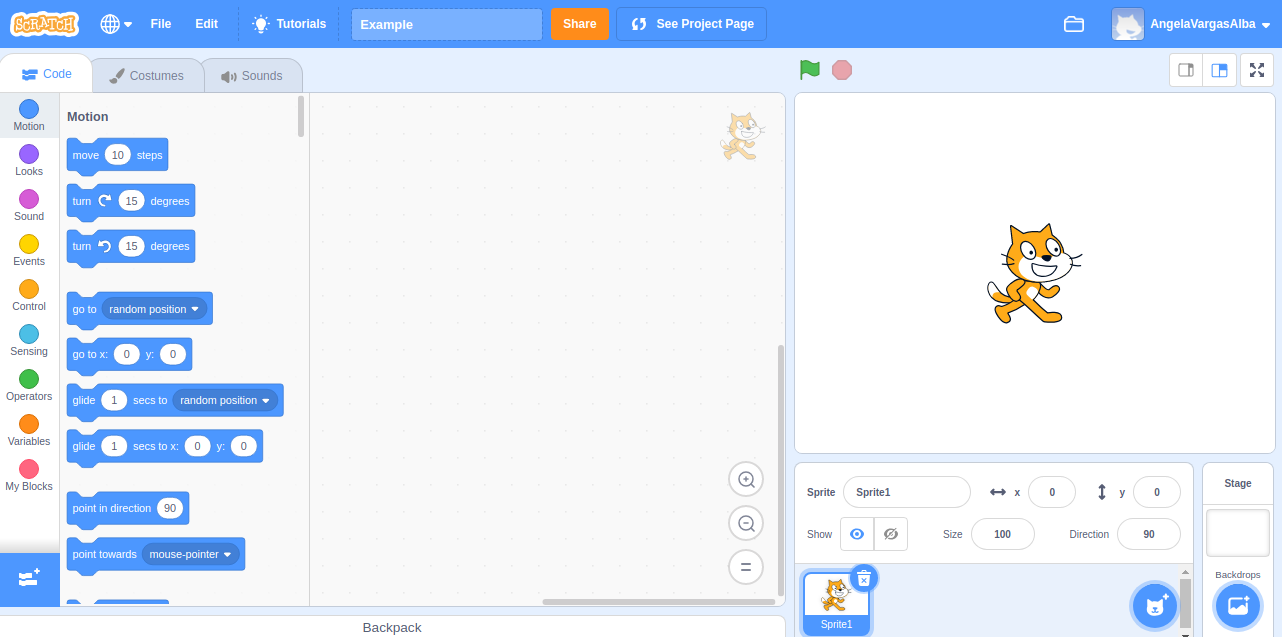
\includegraphics[width=11cm, keepaspectratio]{img/scratch.png}
  \caption{Editor design of Scratch 3.0.}
  \label{fig:scratch}
\end{figure}

On the other hand, Scratch is a world community. In this collaborative space, the ``scratchers'' can interact with each other or share and remix their projects. In addition, they can comment other projects or explain their doubts in a forum. In this way, beginner programmers can learn in a dynamic way, with the help of other programmers with more experience. In Figure~\ref{fig:statistics_scratch} we can observe its statistics in October 2019. Scratch has become an amazing community which also keeps growing. 

\begin{figure}
  \centering
  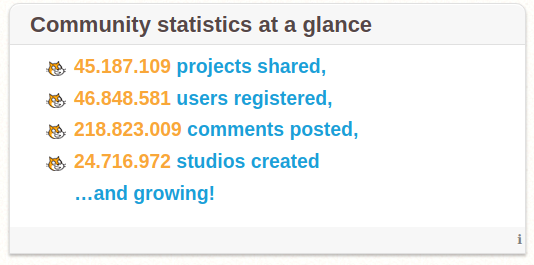
\includegraphics[width=9cm, keepaspectratio]{img/statistics_scratch.png}
  \caption{Statistics of the Scratch community in October 2019.}
  \label{fig:statistics_scratch}
\end{figure}



\section{Frame of reference}
\label{sec:reference}

With the growth of the Scratch community and its impact in the educational field, my tutor of this project - Dr. Gregorio Robles - together with the Dr. Jesús Moreno observed the need of a tool to evaluate the Scratch projects. In this way, Dr. Scratch\footnote{http://www.drscratch.org/} was created in 2014.

Dr. Scratch is a web application which allows both teachers and students to automatize the analysis of Scratch projects. In this way, it helps to verify if the projects have been programmed correctly, to analyze the bad practices in the code, to learn from their errors, to receive feedback or to improve the code. Its main web interface is shown in Figure~\ref{fig:dr_scratch}.

\begin{figure}
  \centering
  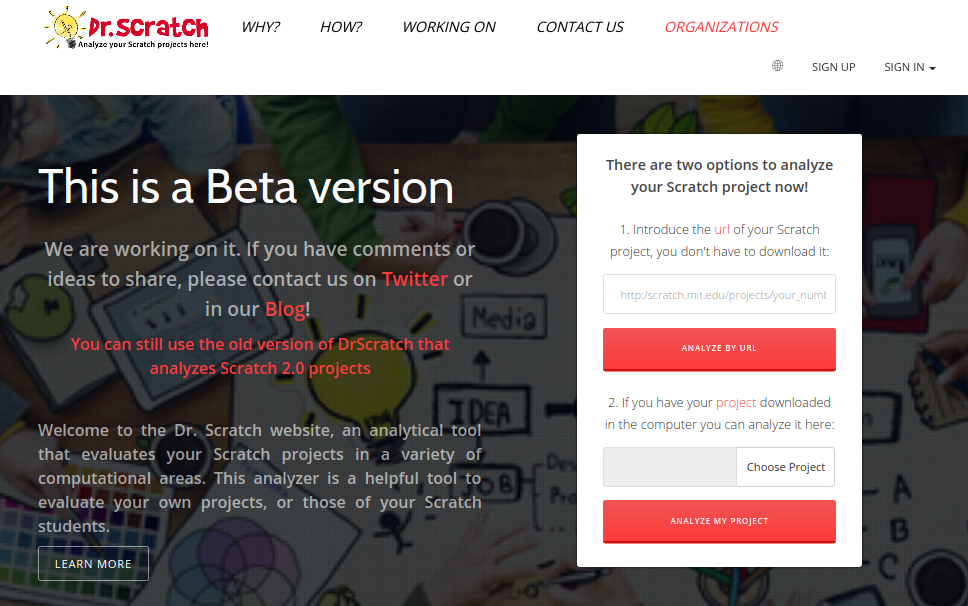
\includegraphics[width=11cm, keepaspectratio]{img/dr_scratch.png}
  \caption{Web interface of the Dr. Scratch tool.}
  \label{fig:dr_scratch}
\end{figure}

For the analysis of the projects, Dr. Scratch used Hairball\footnote{https://github.com/jemole/hairball} in its initial version, a plugin framework which analyzed the files generated with Scratch. These files have a compressed format and contain a JSON file with the relevant information about the blocks utilized in the Scratch projects. In the previous version, Scratch 2.0, the extension of these files was \textit{.sb2}. This format was replaced by the extension \textit{.sb3} in Scratch 3.0. In this way, the content of these JSON files would change significantly and Hairball would not be compatible.

Levering the need to modify the functionality of Hairball to adapt it to the new JSON format, we decided to remove it. The essential objective of this step was to simplify the software of Dr. Scratch, removing Hairball and integrating its new features in the own code of the tool. 

Therefore, the starting point of this project was to adapt Dr.Scratch to the new version Scratch 3.0, which would be launched in the coming months. The challenge of this process was to get the same functionalities, but without the Hairball module.

\hfill

Once the projects are analyzed, Dr. Scratch shows different dashboards with the results of the analysis, which can be observed in Figure~\ref{fig:dashboards}.

\begin{figure}
  \centering
  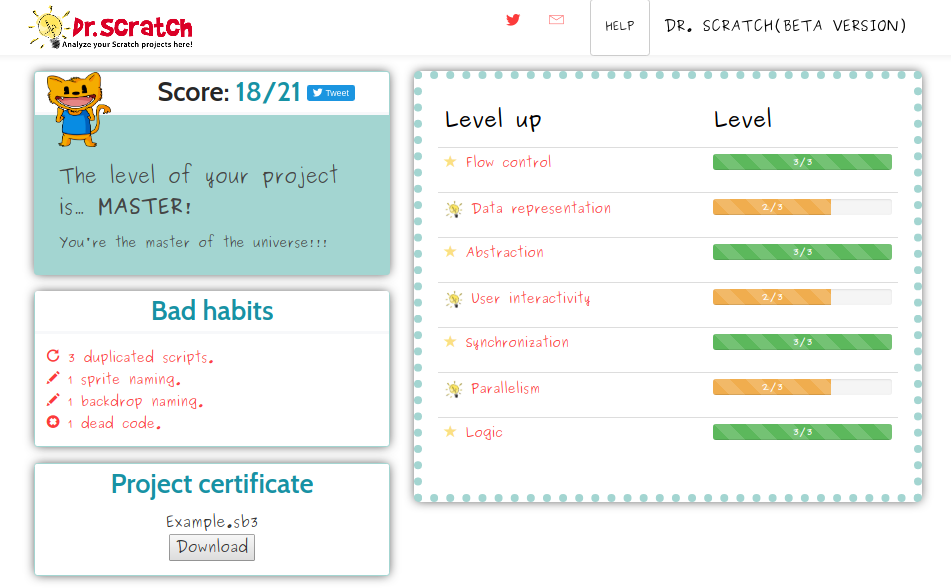
\includegraphics[width=11cm, keepaspectratio]{img/dashboards.png}
  \caption{Dashboard of Dr. Scratch with the results of the analysis.}
  \label{fig:dashboards}
\end{figure}

In order to measure the development grade of CT demonstrated in programming, Dr. Scratch gives a numeric punctuation based on the level reached in each of the seven categories of CT: abstraction, logical thinking, synchronization, parallelism, flow control, user interactivity and data representation~\cite{moreno2015dr}. Each of these capacities receives a punctuation from 0 to 3 points, depending on the Scratch blocks used. In this way, the final score varies between 0 to 21 points, differentiating three different levels of programmers: Basic (0 to 7 points), Developing (8 to 15 points) and Proficiency (16 to 21 points).   

In addition to the CT analysis, Dr.Scratch includes other key functionality in the development of this project: the analysis of bad smells that may exist in the Scratch project. That is, code that has never been executed (dead code), code that is copied and pasted in the scripts of different characters (repeated code) or the lack of significant naming (default naming). However, this dashboard was shown in a small space to the left and in a very summary way.

Another main challenge of this project was to change the importance that bad smells had in Dr. Scratch, in order to raise awareness of their importance. To carry out this process in the most appropriate way, we developed previously an exhaustive analysis about the behaviour of bad smells in Scratch projects.

With this analysis, we could verify that bad smells are present in the majority of the Scratch projects and that they had a negative impact in the development of CT skills. From this point, after a deeper and more exhaustive analysis of them, we considered necessary the development of a new specific model for bad smells in Dr. Scratch. Its final design and implementation can be observed in Figure~\ref{fig:bad_smells_model}.

\begin{figure}
  \centering
  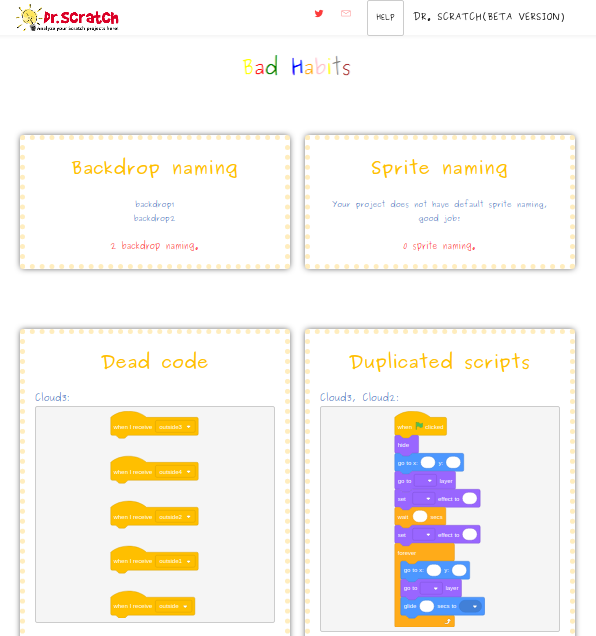
\includegraphics[width=11cm, keepaspectratio]{img/new_model.png}
  \caption{Interface design for the new model of bad smells in Dr. Scratch.}
  \label{fig:bad_smells_model}
\end{figure}

Finally, we found an important weakness in Dr. Scratch during the analysis: It scores positively the presence of bad smells in the Scratch projects. In other words, a project with a larger number and variety of blocks -even these blocks are repeated or dead, for example- will have more punctuation than a simpler project -even it does not have any bad smell. 

From this discovery, we wanted to prove the effectiveness of our analysis with other scenario: the assessment of bad smells in Scratch projects with teachers. In this way, we wanted to verify if teachers develop the same behaviour which we found in Dr. Scratch. 

We developed an experiment in which two teachers of secondary school evaluated six Scratch projects. The experiment was composed of two phases. In both of them they had to analyze and evaluate the same Scratch projects, but firstly in a general way -with any information about bad smells- and, secondly, in a more guided way -receiving information about bad smells. 


\section{Motivation}
\label{sec:motivation}

Nowadays, there is a lack of resources to introduce CT, in particular programming, in the educational field. In many countries is already being implanted this area as a mandatory subject in schools. However, a lot of teachers do not have enough formation to teach in the most appropriate way this academic world. 

Teaching children some good methods of programming and how to avoid bad practices, is one of the most difficult tasks to begin the development of CT. Nowadays, in an era in which programming is at its peak and there is a need to introduce it since childhood, it is very important to do in a responsible and appropriate way since the beginning. 

For this reason, the main motivation of this work has been to analyze in detail the behaviour of bad smells and its evolution. A suitable study about bad smells can help to raise awareness about its presence both in students and teachers, and fostering a more appropriate learning guide.


\section{Structure of the dissertation}
\label{sec:structure}

In order to facilitate the reading of the dissertation, its structure is described in this section. This work is divided into six chapters, which are detailed as follows:

\begin{itemize}
  \item Introduction. This chapter includes a description about the frame of reference of the project, as well as the context in which is involved. Moreover, the main motivation for its realization is explained.
  
  \item Objectives. In Chapter~\ref{chap:objectives}, the general objective is divided into four main different parts. The specific objectives to reach it are also detailed. In addition, a project timeline is included to clarify the planning and organization of all of them.
  
  \item State of the art. We describe the main tools and technologies used during the project in this chapter. In order to facilitate the understanding of them, we have grouped the tools according to the different phases of the project.
  
  \item Design and implementation. This chapter includes the progress of each phase of the project and the implementation of the different tools described. The development of the bad smells analysis, as well as the previous and subsequent processes that have been needed, will be detailed in this section. 
  
  \item Results. In this chapter, we mainly describe the results obtained from the bad smells analysis. We answer the research questions raised in the project and analyze the results found. In addition, we show the results from the assessment experiment developed.
  
  \item Conclusions. In this final chapter, we draw conclusions and hint to ideas that could be used for further research.
  
\end{itemize}

